\chapter{Solution Proposal}
\label{sec:solution_proposal}

This chapter will define the problem, establish how success will be evaluated, define the methodology for developing the solution, and present the associated risks.

\section{Problem definition}


The challenge is to design and develop a comprehensive system that can effectively process, validate, and aggregate voluntary contributions supported by various types of data. This system would need to be able to classify the severity of forest fire events based on aggregated data.

Moreover, it would need to identify the geolocation and track the temporal evolution of a wildfire event. Providing properly organised and validated information is crucial, as it can help increase knowledge about the event, facilitate real-time decision-making, and potentially save lives and resources.


Finally, the system would need a set of plotting tools to aid in information gathering and posterior analysis.



Figure \ref{fig:mockup_presentation} shows in rudimentary way, multiple geographic location that don't have correlation to each other. Each tile represents a different biome, and each one is named after a letter. Fire risk is composed of four distinct categories, red which is associated with extreme risk of fire, orange is high risk, yellow is moderate risk, and green is low risk of fire.
Tile C is on the worst-risk. There are several active fire fronts, and it is windy. 


Tile A has high risk and has a forest near a rural area, this may have enhanced fire ignition due to human activities. Tile B is near a town, but since it isn't windy or very hot, it has a moderate risk of fire. Tile D is the least likely to catch on fire, it is raining and the weather is cold. It has a risk score of green signalling a low risk of fire.


This imaginary exercise can be converted into the real world, because it entangles the problem at its core. Create a fire risk and occurrence analysis with multiple sources of data and then show it in a easy manner.


The tiles would be geographical areas, and risk would be associated with it given each region's fire influencing factors.


In essence, the goal is to create a comprehensive system that can handle a wide range of data types, make sense of this data, and provide actionable insights about forest fire events.


\begin{figure}[h!]
 \centering
  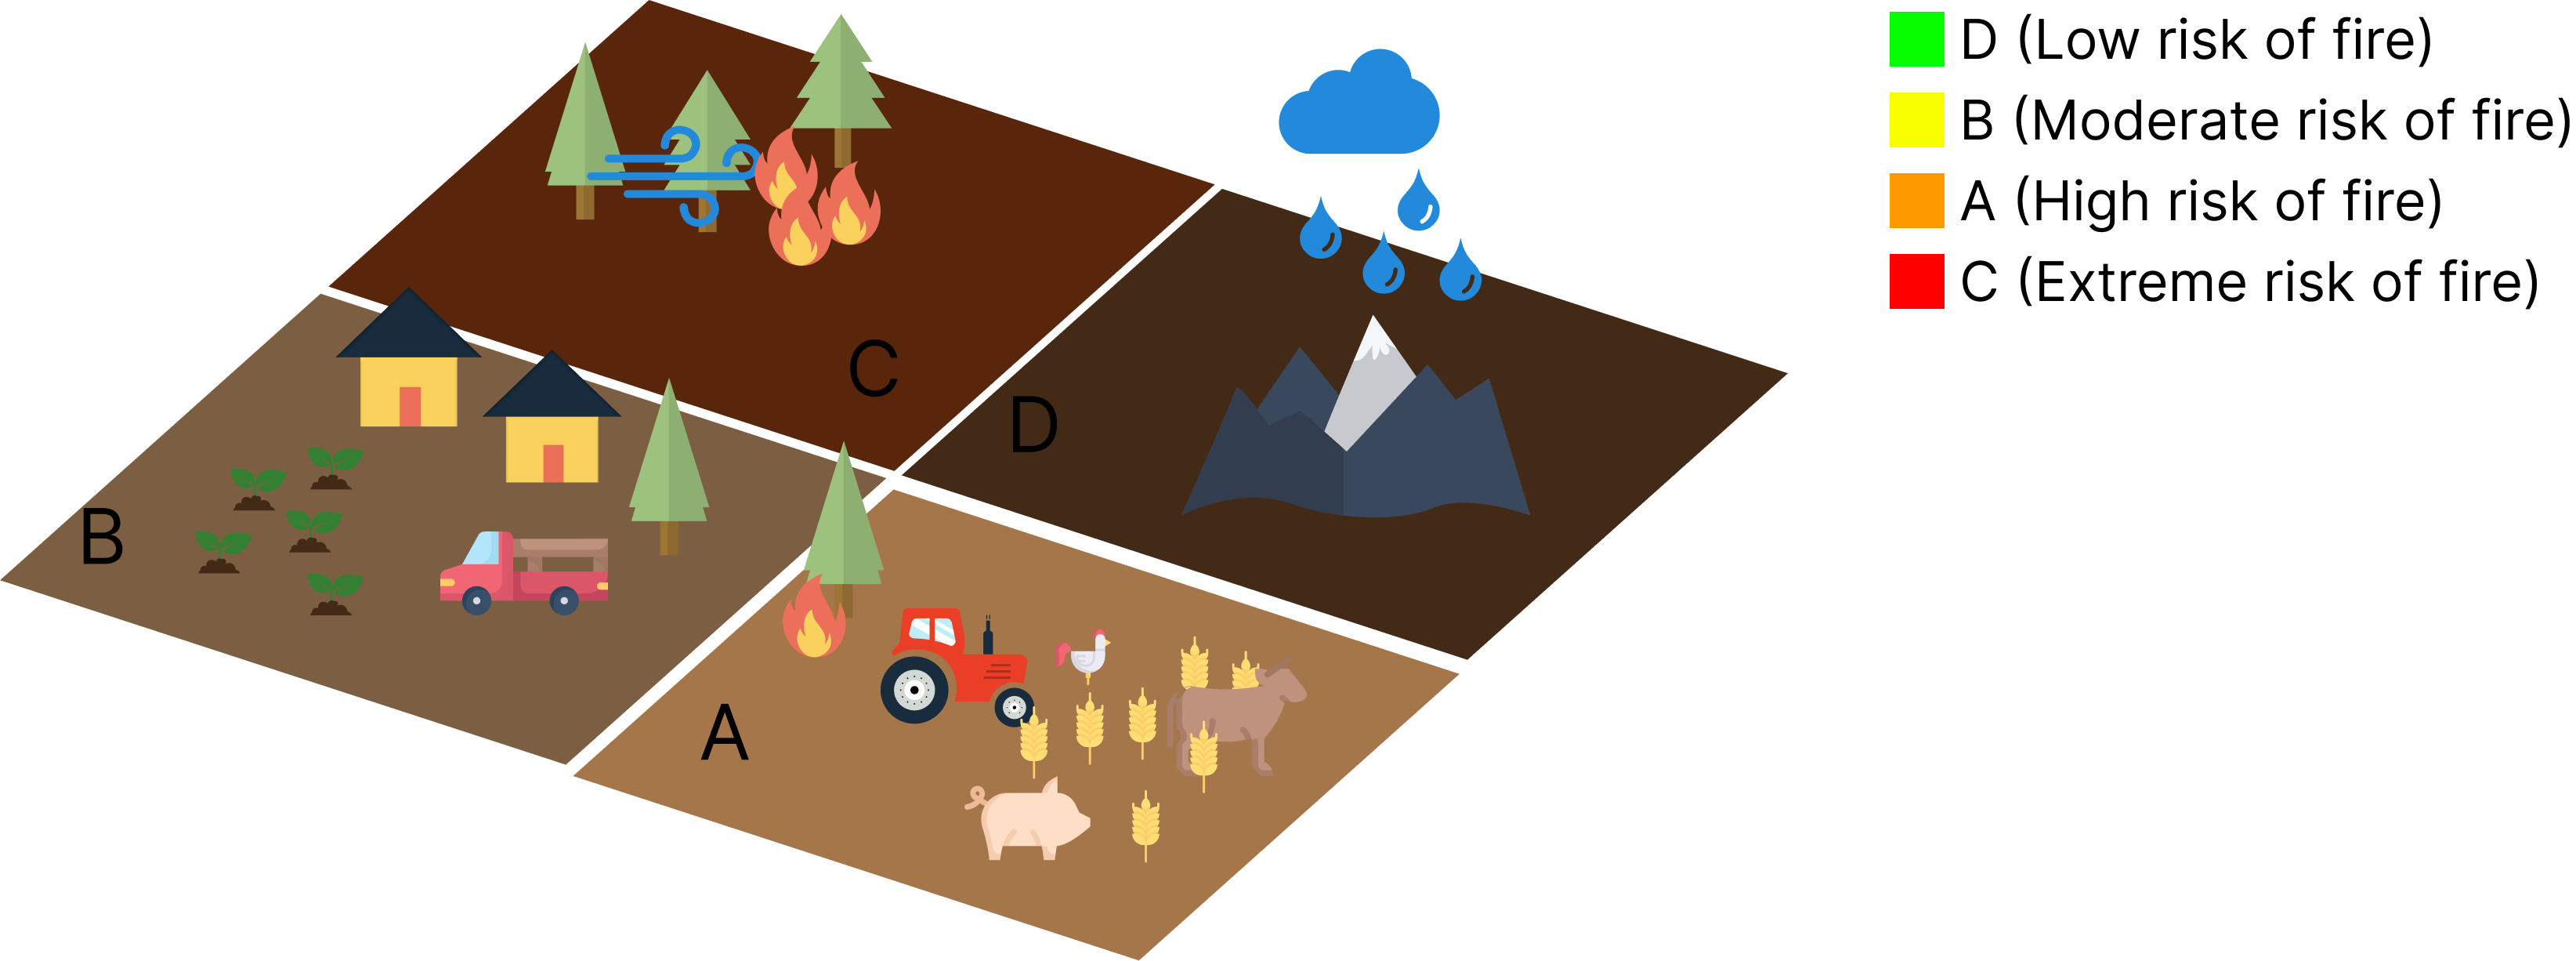
\includegraphics[width=1.0\linewidth]{frontmatter/imgs/Group 1.png}
  \caption{Tiles depicting geographical areas and forest fire risk}
  \label{fig:mockup_presentation}
\end{figure}

\section{Proposed Methodology}
The methodology section will cover the steps for carrying out the solution. Firstly, data is collected from various sources to create a data pipeline. This is followed by the step of merging the data according to its features. The fusion can be done recursively until there is satisfaction with the information obtained.


The data will be combined with other external sources, and depending on the scarcity of the data, it may be necessary to generate synthetic data. Once the data has been cleaned, it will be placed in a database.


The models will use the database to obtain classification results. The results will focus on risk, susceptibility, and fire occurrence. Finally, with the help of data visualisation tools, the findings will be displayed.

\subsection{Data Pipeline} 
Data pipeline is the process of extracting, transforming, and loading data from diverse sources, such as volunteer contributions, geographical data, and meteorological data. The following steps comprise the data pipeline:

\subsubsection{Data extraction}
Data is gathered from a variety of sources, including websites, APIs, and databases.

\subsubsection{Data transformation}
Following extraction, the data is cleaned (duplicates are removed and missing values are handled), normalized (ensuring that is in a consistent format), and enriched. 

\subsubsection{Data loading}
The transformed data is then loaded into an appropriate data storage system, such as a database. This enables efficient searching and retrieval of data when it is required for analysis.

\subsection{Data Fusion}
Data fusion can happen at the data transformation step. At this level, decision-level and feature-level fusion will occur (see \ref{data_fusion} for a more detailed explanation of each one).

\subsection{Data enhancement}
Data enhancement follows the fusion step. At this level, data can be enriched with external sources or generated.


\subsection{Classification Models}
Experiments will be conducted on data with multiple machine learning models to convey the ones with better metrics and performance and highlight the most useful features in forest fire event classification. For fire occurrence, Random Forest and SVM are strong candidates for a first approach. These two models are easy to implement and highlighted high results in \cite{9726029} and \cite{SAYAD2019130}. For fire risk, an ANN model is the strongest candidate, as shown in \cite{rs13132513}.

\subsection{Data Visualisation}
Data visualisation will enable the plotting and presentation of forest fire severity classification results, as well as the display of aggregated and validated information.


\subsection{Outcome}
The project's output would be the information derived from the classification models. If in a given area or given some meteorological indices, the system will determine the likelihood of fire (fire or no fire) and the associated risk (low, moderate, high, or extreme). This information will be presented using data visualisation tools.


\section{Planning and organisation}
Figure \ref{fig:gantt_first} exhibits the time taken for each step in the first semester. It has a comparison between the time expected for each task and the actual time taken to complete it. The comprising steps in the first Gantt chart are:
\begin{enumerate}
    \item Learn Key Concepts - Forest Fire Management, Issues, Decision Support systems;
    \item Learn Key Concepts - Machine learning applied to forest fire, Mathematical models, and Influencing factors;
    \item Learn models used to classify Forest Fire;
    \item Research data visualisation tools and libraries;
    \item Study of the problem;
    \item Define the solution, objectives, success criteria, risks and methodology;
    \item Write document.
\end{enumerate}


Figure \ref{fig:gantt_second} shows the proposed Gantt chart for the second semester. The following list will explain each step in figure \ref{fig:gantt_second}:

\begin{enumerate}
    \item Collect data from multiple sources: The first step involves the gathering of multiple data sources;
    \item Extract, Transform, and Load Data: Apply extract, transform, and load techniques to the gathered data. In this step, the data pipeline is created.
    \item Fusion techniques on data: This step undertakes the fusion methodologies inside the pipeline;
    \item Conduct forest fire event classification with RF and ANN models: Random forest and ANN have been chosen as the first candidates to tackle the problem of forest fire occurrence and risk;
    \item Utilise fused and classification outputs to visualise the information: This is regarded as the last step in the system's implementation. The findings discovered in the previous steps are now interpretable information ready to be used in a decision-support system;
    \item Assemble the scientific paper: Besides the thesis, this project should result in a scientific paper;
    \item Write document: The last step is the completion of the thesis document.
\end{enumerate}

\begin{figure}[h!]
 \centering
  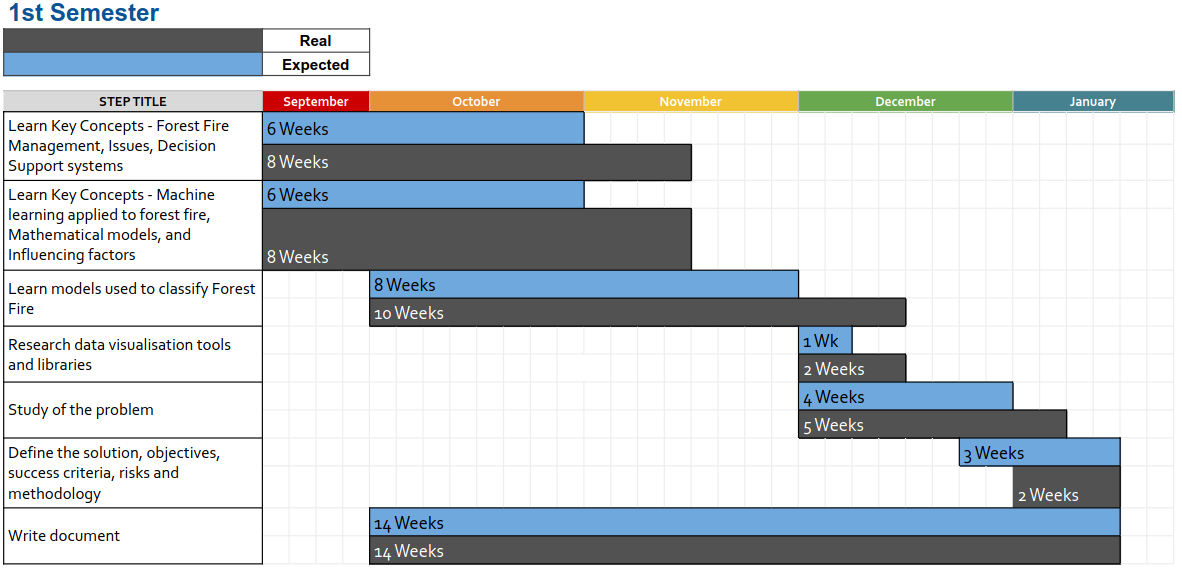
\includegraphics[width=1.0\linewidth]{frontmatter/imgs/g1.png}
  \caption{Gantt chart for first semester}
  \label{fig:gantt_first}
\end{figure}

\begin{figure}[h!]
 \centering
  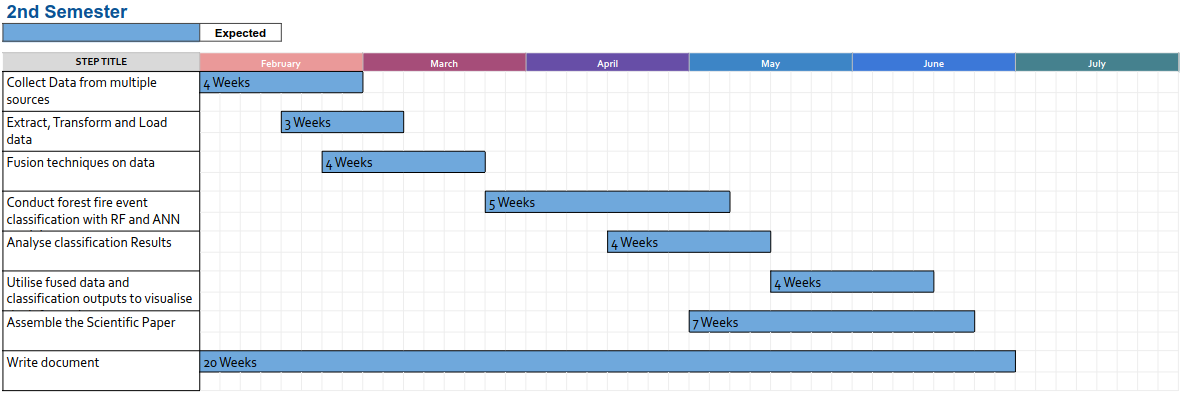
\includegraphics[width=1.0\linewidth]{frontmatter/imgs/g2.png}
  \caption{Proposed gantt chart for the second semester}
  \label{fig:gantt_second}
\end{figure}


\section{Risk analysis}
In this section, the potential risk that may affect the success of the approach is identified, and mitigation and impact plans for the risk are proposed. A qualitative probability and impact level were also assigned using the following scales: low, medium, and high. Table \ref{risk_du} outlines the only identified risk.

\begin{table}[h!]
\caption{Risk - Data unavailability}
\label{risk_du}
\begin{tabular}{|p{2cm}|p{12cm}|}
\hline
Risk            & Data unavailability \\ \hline
Description     & Due to technological challenges, privacy limitations, or other factors, some data sources may not be available. \\ \hline
Mitigation Plan & To provide data redundancy and variety, many data sources are employed.  \\ \hline
Impact Plan     & Identify alternative data sources. Generate data. Adapt the prediction model to work effectively with the available data. Adapt the experiment to the available data. \\ \hline
Probability     & High \\ \hline
Impact          & High \\ \hline
\end{tabular}
\end{table}


\section{Success Evaluation Criteria}
The success of the project can be measured in two dimensions: the realisation of the proposed objectives and how closely the outcomes resemble reality. That is, whether the system is able to assess whether there is a likelihood of fire or not. Also, regarding success outcomes, data visualisation should play a key role in showing findings in a clean manner. Therefore, the following steps must be considered when evaluating the success of the outcomes:

\subsection{Classification performance}
The classification model's accuracy, precision, recall, F1-score, and AUC will be evaluated. The models will be also compared to other classification results and sources on historical data. 
Different machine learning algorithms' performance will be examined, and feature selection approaches will be utilised to discover the best model and the most significant characteristics for the classification problem.


\subsection{Visualization effectiveness}
The visualisation should be simple, and easy to follow. This can be achieved by following design guidelines and making comparisons with other data visualisation interfaces. 


